\documentclass[]{article}

\usepackage{graphicx}
\usepackage{url}
\usepackage{hyperref}

%opening
\title{Master Thesis: Real-time streamsurface computation}

\date{March 15, 2016}

\begin{document}

\maketitle

\begin{description}
	\centering
	\item[] \textbf{Supervisor}: Prof.Dr. Ruediger Westermann
	\item[] \textbf{Advisors}: Dr. Andreas Dietrich, Dr. Frank Michel\newline{}%
\end{description}


\begin{abstract}

Streamsurfaces are one of the powerful visualization tools, which are used to gain insight into characteristics and features of flow fields. In practice, streamsurfaces are approximated by triangulating adjacent pairs of integral curves, originating from a seeding line. The generation of integral curves bears quite some similarities to ray tracing algorithms used in physically based renderers. Although, the techniques used in ray tracing may not have good performance in the streamline computation context due to their different computational nature, they can be optimized for streamline computation by introducing some modifications. In this master thesis, I present my work on accurate streamsurface computation and rendering in real-time, by exploiting the scalability and portability features of parallel architectures in heterogeneous computing, and utilizing concepts from physically based rendering. To improve the efficiency, I use a scheduler to divide the streamsurface computation and rendering tasks on different devices proportional to their computation powers. Additionally, I apply and evaluate different acceleration structures and the concepts of caching to improve the efficiency and utilization of streamsurface generation on modern GPUs and CPUs to achieve real-time results. Furthermore, the possible impact of applying ray-packing and ray-sorting to the streamline computation is investigated.\newline

Implemented using OpenCL, OpenGL 4.5, and C++.\newline

More information can be found on:\

\href{https://mmostajab.com/master-thesis-d/}{https://mmostajab.com/master-thesis-d/}

\end{abstract}



\begin{figure}[!ht]
	\centering
	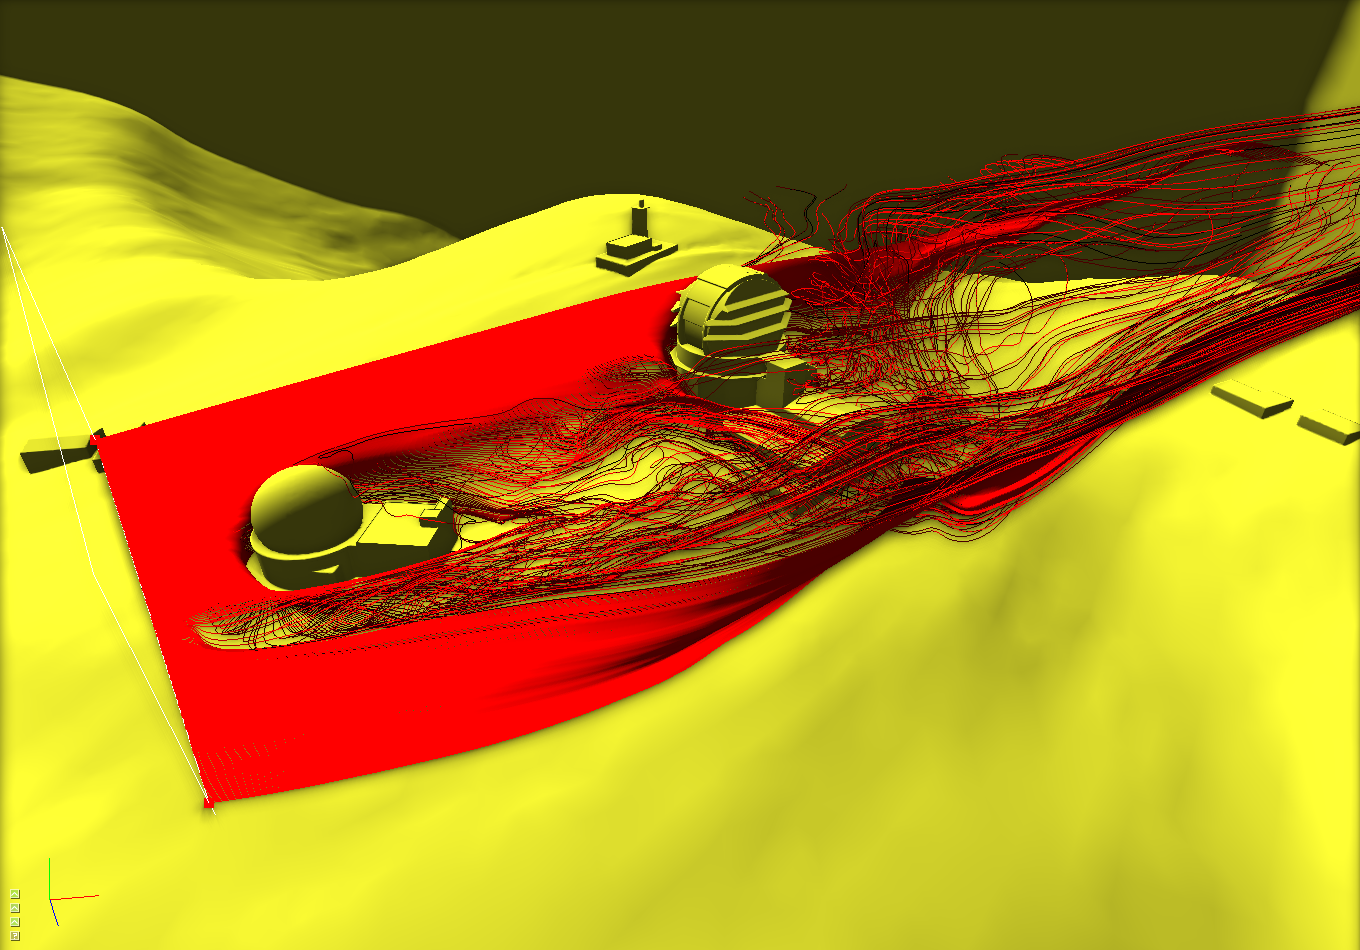
\includegraphics[width=0.80\textwidth]{telescope}
	\caption[Streamlines in telescope dataset]{\textbf{Streamlines in telescope dataset}. one thousands streamlines integrated 5000 steps on the CPU. The result is rendered with screen space ambient occlusion (SSAO). }
	\label{fig:telescope_result}
\end{figure}


\begin{figure}[!ht]
	\centering
	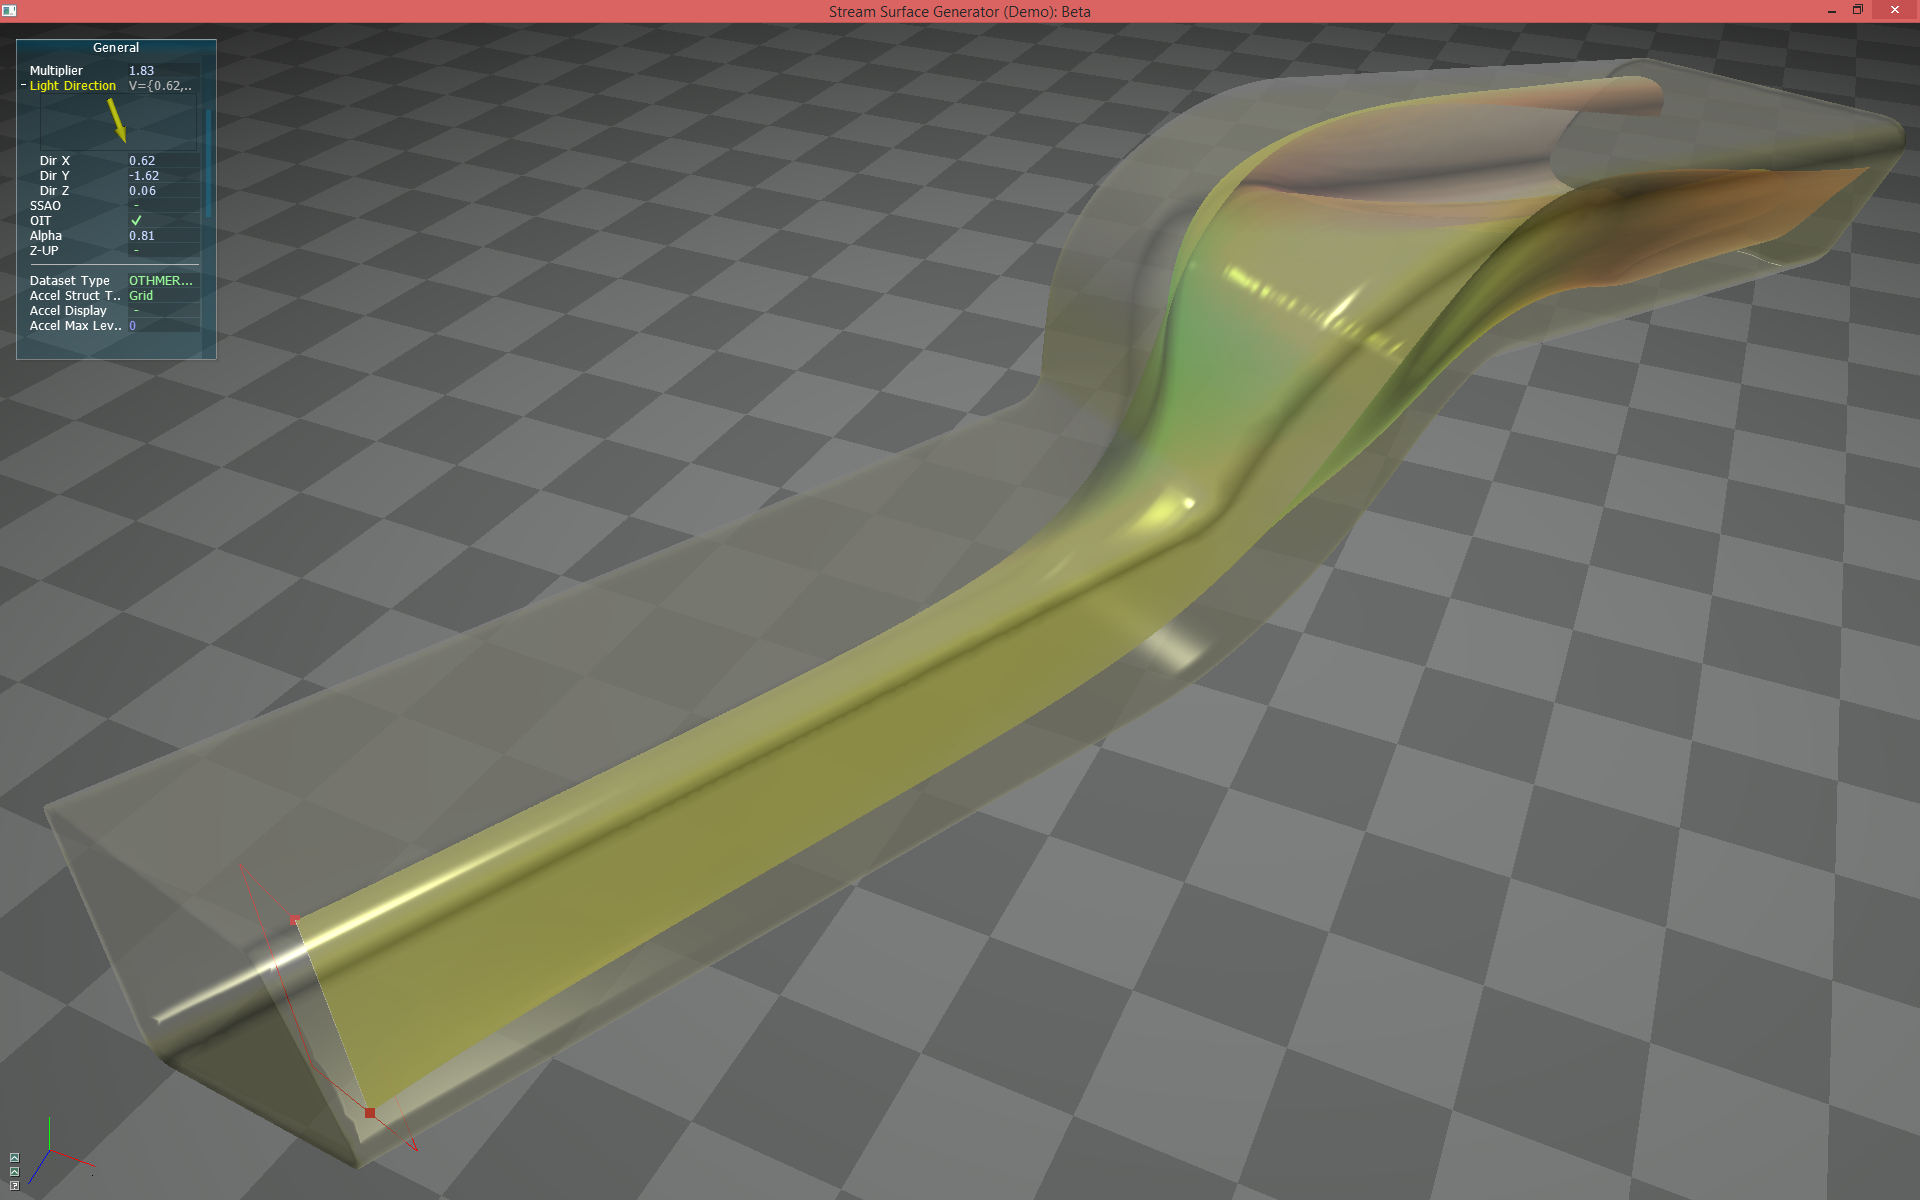
\includegraphics[width=0.80\textwidth]{othmer.png}
	\caption[Streamsurface in wind tunnel dataset]{\textbf{Streamsurface in wind tunnel dataset}. Streamsurface made of 1000 streamlines integrated 1000 steps in the wind tunnel dataset. The result output is rendered with transparency.}
	\label{fig:othmer_result}
\end{figure}

\begin{figure}[!ht]
	\centering
	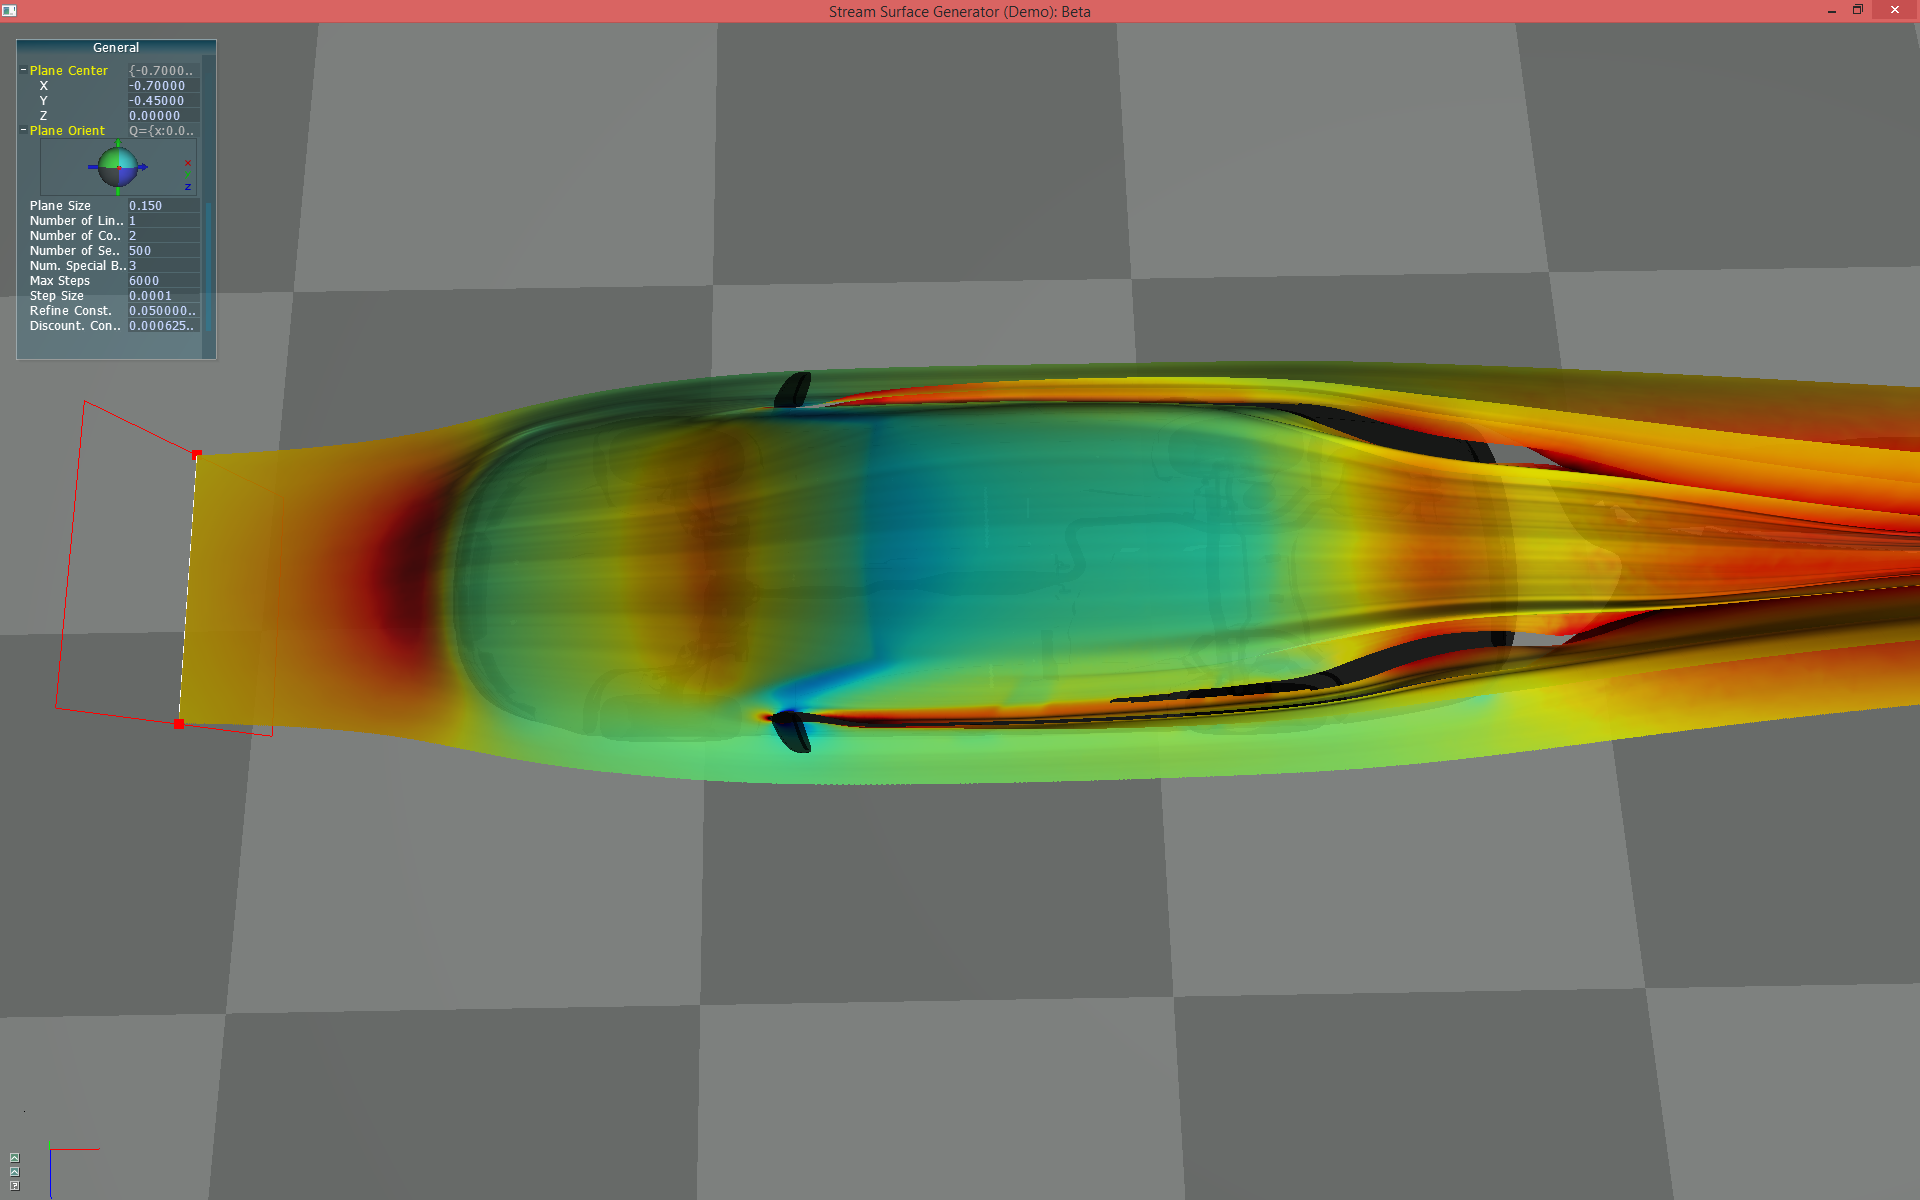
\includegraphics[width=0.80\textwidth]{car.png}
	\caption[Streamsurface in car dataset]{\textbf{Streamsurface in car dataset}. Streamsurface made by 1000 streamlines integrated 1000 steps in car dataset. The velocity length on the streamsurface is mapped to Jet colormap.}
	\label{fig:car_result}
\end{figure}


\begin{figure}[!ht]
	\centering
	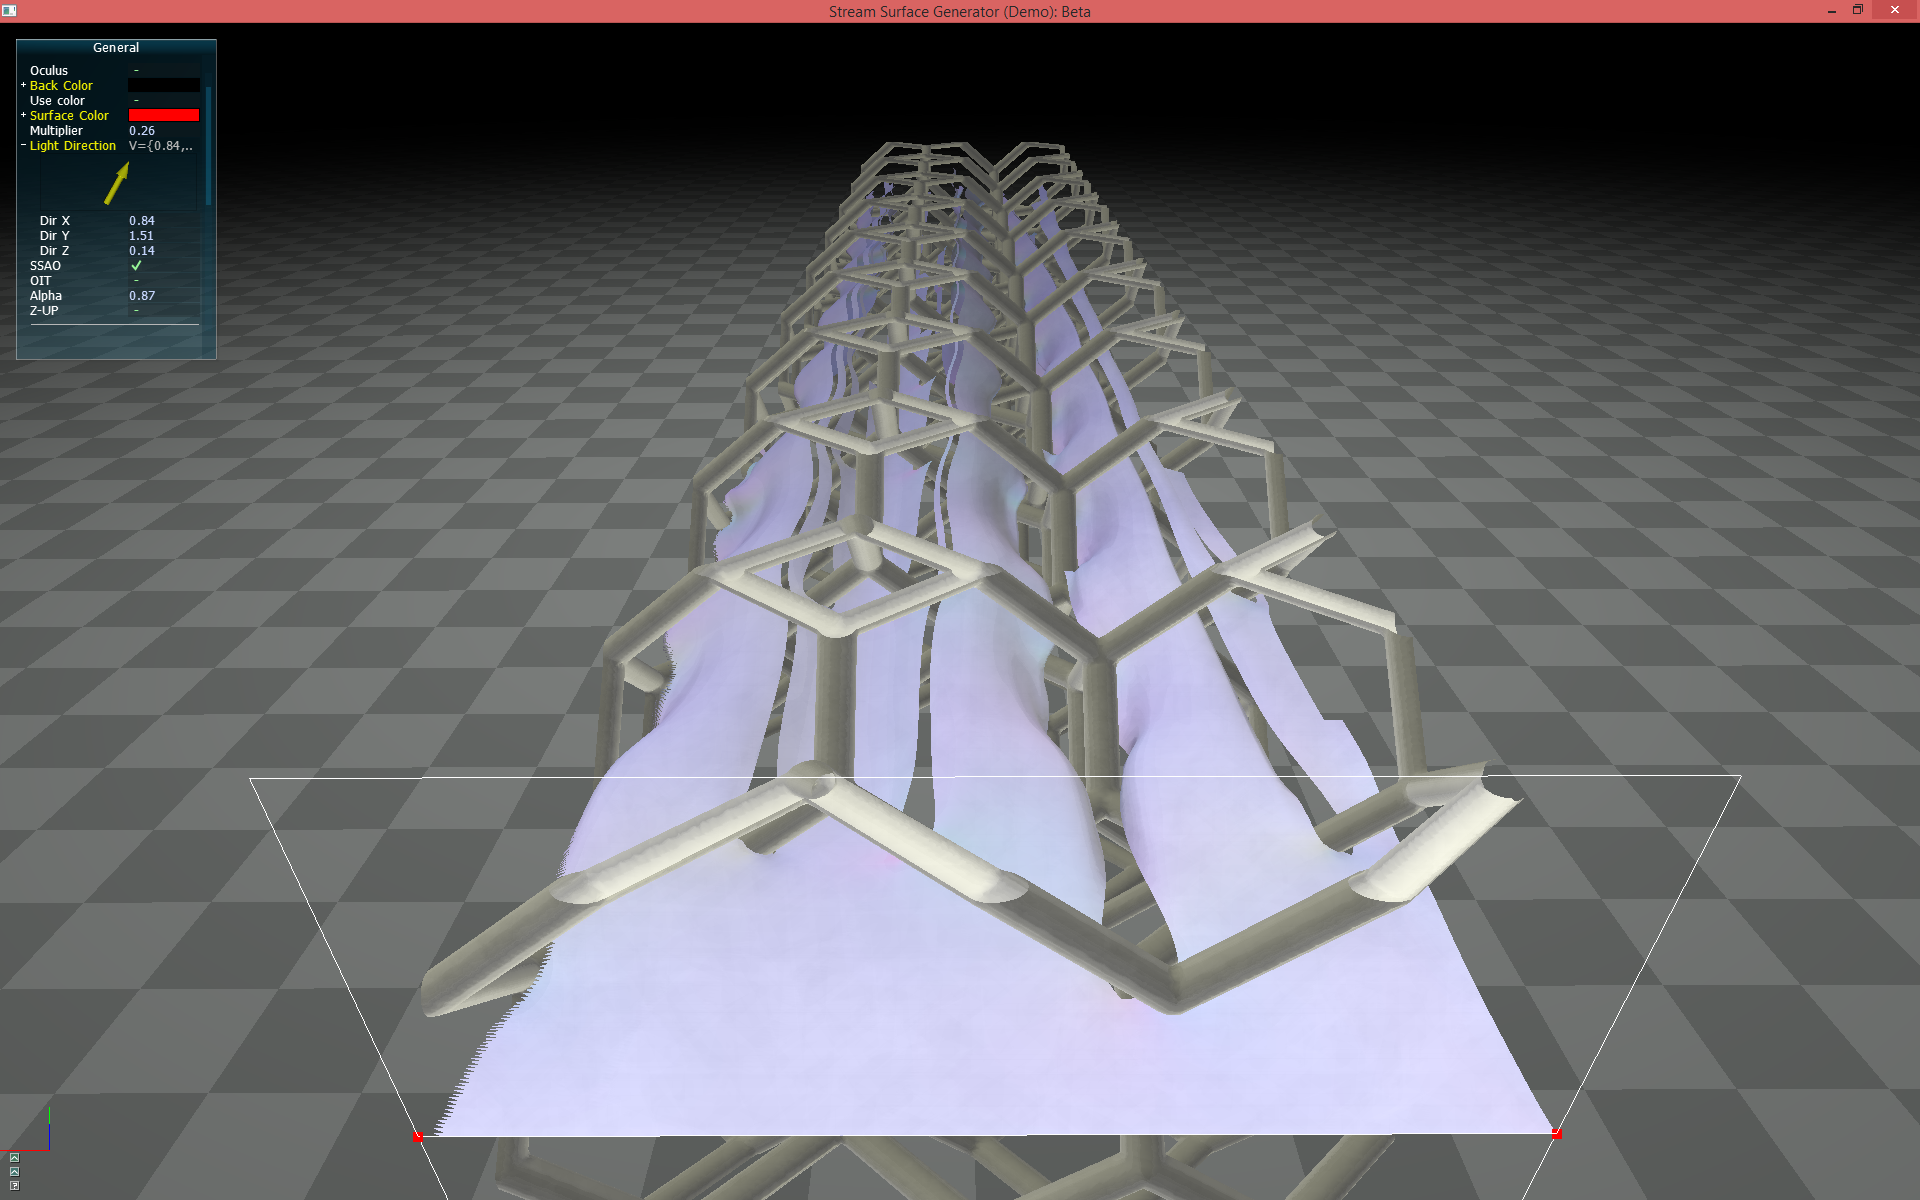
\includegraphics[width=0.80\textwidth]{tetra.png}
	\caption[Streamsurface in tetrahedradecal dataset]{\textbf{Streamsurface in tetrahedradecal dataset}. Streamsurface made by 1000 streamlines integrated 1000 steps in tetrahedradecal dataset.  }
	\label{fig:tetra_result}
\end{figure}

\end{document}
